\documentclass[tikz,border=5pt]{standalone}

\usepackage[T1]{fontenc}
\usepackage{lmodern}
\usepackage{amssymb}
\usepackage{fontawesome5}
\usepackage{xcolor}
\usetikzlibrary{arrows.meta,calc,positioning,shapes.geometric}

\definecolor{SourceBlue}{HTML}{148DD1}
\definecolor{SourceBlueDark}{HTML}{075E9A}
\definecolor{SourcePaleBlue}{HTML}{EAF6FC}
\definecolor{SourceGreen}{HTML}{14A83B}
\definecolor{SourcePaleGreen}{HTML}{E5F8E9}
\definecolor{SourceRed}{HTML}{EF3340}
\definecolor{SourcePaleRed}{HTML}{FFF0F1}
\definecolor{SourceYellow}{HTML}{FFF0B3}
\definecolor{SourceGrey}{HTML}{F0F0F0}

\begin{document}
\begin{tikzpicture}[
  x=1cm,
  y=1cm,
  font=\sffamily,
  >={Latex[length=2.2mm,width=1.4mm]},
  flow/.style={->, draw=black, line width=0.55pt},
  leakflow/.style={->, draw=SourceBlue, line width=0.8pt},
  leaklabel/.style={fill=white, inner sep=2pt, text=SourceBlueDark,
    font=\bfseries\fontsize{7}{8}\selectfont},
  panel/.style={draw=black, line width=0.75pt, rounded corners=3mm, fill=white},
  sxcard/.style={rectangle, draw=black!55, line width=0.55pt, rounded corners=1.2mm,
    fill=SourcePaleBlue, minimum width=2.55cm, minimum height=2.75cm,
    inner sep=1.5mm, align=center},
  sxsuccess/.style={sxcard, fill=SourcePaleGreen},
  report/.style={fill=SourcePaleBlue, rounded corners=1.5mm,
    minimum width=8.7cm, minimum height=1.00cm, align=center},
  title/.style={font=\rmfamily\fontsize{13}{15}\selectfont},
  number/.style={font=\rmfamily\fontsize{12}{14}\selectfont},
  steptitle/.style={font=\sffamily\bfseries\fontsize{8.3}{9.5}\selectfont,
    text width=2.20cm, inner sep=0pt, align=center},
  stepbody/.style={font=\rmfamily\fontsize{7.4}{8.4}\selectfont,
    text width=2.20cm, inner sep=0pt, align=center},
  narrowtitle/.style={steptitle, text width=1.90cm},
  narrowbody/.style={stepbody, text width=1.90cm},
  icon/.style={font=\bfseries\fontsize{18}{19}\selectfont, text=SourceBlue},
  smallnote/.style={font=\rmfamily\fontsize{6.8}{8.0}\selectfont, align=center}
]

% -----------------------------------------------------------------------------
% Panel 1: Distribute and record
% -----------------------------------------------------------------------------
\draw[panel] (0,8.55) rectangle (18.3,13.35);
\node[number, anchor=west] at (0.55,12.90) {01};
\node[title, anchor=west] at (1.95,12.90) {DISTRIBUTE \& RECORD};

% Avoid TikZ's built-in `step` key: it controls grid spacing.
\node[sxcard] (register) at (1.60,11.20) {};
\node[sxcard] (encrypt)  at (4.60,11.20) {};
\node[sxcard] (wrap)     at (7.60,11.20) {};
\node[sxcard] (decrypt)  at (10.60,11.20) {};
\node[sxcard] (mark)     at (13.60,11.20) {};
\node[sxsuccess] (commit) at (16.60,11.20) {};

\node[icon] at ($(register.center)+(0,0.72)$) {\faIcon{file-upload}};
\node[icon] at ($(encrypt.center)+(0,0.72)$) {\faIcon{lock}};
\node[icon] at ($(wrap.center)+(0,0.72)$) {\faIcon{key}};
\node[icon] at ($(decrypt.center)+(0,0.72)$) {\faIcon{unlock-alt}};
\node[icon] at ($(mark.center)+(0,0.72)$) {\faIcon{file-signature}};
\node[circle, fill=SourceGreen, text=white, minimum size=7mm,
  font=\bfseries\fontsize{15}{15}\selectfont] at ($(commit.center)+(0,0.72)$) {\(\checkmark\)};

\node[steptitle] at ($(register.center)+(0,0.05)$) {Register PDF};
\node[stepbody] at ($(register.center)+(0,-0.68)$) {SHA3-256\\original hash};

\node[steptitle] at ($(encrypt.center)+(0,0.05)$) {Encrypt Once};
\node[stepbody] at ($(encrypt.center)+(0,-0.68)$) {AES-256-GCM};

\node[steptitle] at ($(wrap.center)+(0,0.05)$) {Wrap CEK};
\node[stepbody] at ($(wrap.center)+(0,-0.68)$) {ML-KEM-768\\HKDF + AES-GCM\\wrap same CEK};

\node[steptitle] at ($(decrypt.center)+(0,0.05)$) {Decrypt};
\node[stepbody] at ($(decrypt.center)+(0,-0.68)$) {Recover CEK\\then decrypt PDF};

\node[steptitle] at ($(mark.center)+(0,0.05)$) {Mark + Sign};
\node[stepbody] at ($(mark.center)+(0,-0.68)$) {Mark + file hash\\ML-DSA-65 signs event};

\node[steptitle] at ($(commit.center)+(0,0.05)$) {Commit + Deliver};
\node[stepbody] at ($(commit.center)+(0,-0.68)$) {2-of-3 signed quorum\\then download};

\draw[flow] (register.east) -- (encrypt.west);
\draw[flow] (encrypt.east) -- (wrap.west);
\draw[flow] (wrap.east) -- (decrypt.west);
\draw[flow] (decrypt.east) -- (mark.west);
\draw[flow] (mark.east) -- (commit.west);

\node[fill=SourceGrey, rounded corners=1.2mm, minimum width=17.55cm,
  minimum height=0.65cm, smallnote] at (9.15,9.05)
  {Each decryption creates a new session and an image-only PDF with a unique visual watermark.};

% Draw the suspected-copy connector after both panels, so it stays visible.

% -----------------------------------------------------------------------------
% Panel 2: Investigate and verify
% -----------------------------------------------------------------------------
\draw[panel] (0,0) rectangle (18.3,6.95);
\node[number, anchor=west] at (0.55,6.35) {02};
\node[title, anchor=west] at (1.95,6.35) {INVESTIGATE \& VERIFY};

\node[sxcard, minimum width=2.20cm, minimum height=2.65cm] (upload) at (1.55,4.50) {};
\node[sxcard, minimum width=2.20cm, minimum height=2.65cm] (detect) at (4.05,4.50) {};
\node[sxcard, minimum width=2.20cm, minimum height=2.65cm] (evidence) at (6.55,4.50) {};
\node[sxcard, minimum width=2.60cm, minimum height=2.65cm] (verify) at (9.35,4.50) {};

\node[icon] at ($(upload.center)+(0,0.68)$) {\faIcon{file-upload}};
\node[icon] at ($(detect.center)+(0,0.68)$) {\faIcon{search}};
\node[icon] at ($(evidence.center)+(0,0.68)$) {\faIcon{database}};
\node[icon] at ($(verify.center)+(0,0.68)$) {\faIcon{tasks}};

\node[narrowtitle] at ($(upload.center)+(0,0.02)$) {Upload PDF};
\node[narrowbody] at ($(upload.center)+(0,-0.70)$) {Suspected copy};

\node[narrowtitle] at ($(detect.center)+(0,0.02)$) {Detect Mark};
\node[narrowbody] at ($(detect.center)+(0,-0.70)$) {Reference image\\pixel correlation};

\node[narrowtitle] at ($(evidence.center)+(0,0.02)$) {Load Evidence};
\node[narrowbody] at ($(evidence.center)+(0,-0.70)$) {Session +\\signed event};

\node[steptitle, text width=2.30cm] at ($(verify.center)+(0,0.10)$) {Verify Proofs};
\node[stepbody, text width=2.30cm, anchor=north,
  font=\rmfamily\fontsize{6.9}{7.5}\selectfont]
  at ($(verify.center)+(0,-0.18)$)
  {Event + mark\\Recipient + validator\\signatures + chain\\2-of-3 quorum};

\node[diamond, draw=black!70, fill=SourceYellow, aspect=1.45,
  minimum width=2.10cm, minimum height=1.45cm,
  font=\bfseries\fontsize{7.0}{8.0}\selectfont, align=center] (decision) at (12.55,4.50)
  {All checks\\pass?};

\node[draw=SourceGreen, fill=SourcePaleGreen, rounded corners=1.2mm,
  minimum width=3.35cm, minimum height=2.20cm, align=center] (match) at (16.20,4.65) {};
\node[circle, fill=SourceGreen, text=white, minimum size=8mm,
  font=\bfseries\fontsize{17}{17}\selectfont] at ($(match.center)+(0,0.62)$) {\(\checkmark\)};
\node[steptitle, text width=2.90cm] at ($(match.center)+(0,-0.05)$) {VERIFIED MATCH};
\node[stepbody, text width=2.90cm] at ($(match.center)+(0,-0.65)$) {Recipient + session\\Copy attribution};

\node[draw=SourceRed, fill=SourcePaleRed, rounded corners=1.2mm,
  minimum width=5.10cm, minimum height=0.95cm, align=center] (invalid) at (12.55,2.65) {};
\node[circle, fill=SourceRed, text=white, minimum size=6.2mm,
  font=\bfseries\fontsize{12}{12}\selectfont] at ($(invalid.west)+(0.45,0)$) {!};
\node[steptitle, text width=4.05cm,
  font=\sffamily\bfseries\fontsize{8}{9}\selectfont]
  at ($(invalid.center)+(0.35,0.18)$) {INCONCLUSIVE / INVALID};
\node[stepbody, text width=4.05cm] at ($(invalid.center)+(0.35,-0.23)$) {UNAVAILABLE};

\draw[flow] (upload.east) -- (detect.west);
\draw[flow] (detect.east) -- (evidence.west);
\draw[flow] (evidence.east) -- (verify.west);
\draw[flow] (verify.east) -- (decision.west);
\draw[flow] (decision.east) -- node[above, font=\bfseries\fontsize{6.5}{7}\selectfont] {YES} (match.west |- decision.east);
\draw[flow] (decision.south) -- node[right, font=\bfseries\fontsize{6.5}{7}\selectfont] {NO} (invalid.north);

\node[report] (report) at (8.65,1.40) {};
\node[icon, font=\fontsize{16}{17}\selectfont] at ($(report.west)+(0.65,0)$) {\faIcon{file-alt}};
\node[steptitle, text width=6.6cm, align=left, anchor=west]
  at ($(report.west)+(1.30,0.22)$) {Investigation Report};
\node[stepbody, text width=6.6cm, align=left, anchor=west]
  at ($(report.west)+(1.30,-0.25)$)
  {Evidence checks; no claim about who leaked it};

% Both outcomes create a report. The auditor reviews the ledger evidence.
\draw[flow] (invalid.south) -- (12.55,2.02)
  -- (10.60,2.02) -- (10.60,1.90);
\draw[flow] (match.south) |- (report.east);
\node[stepbody, text width=3.2cm] at (14.90,0.98)
  {Auditor review:\\ledger + audit trail};

% Route outside the note strip and along the panel margin, never over a heading.
\draw[leakflow] (commit.east) -- (18.10,11.20)
  -- (18.10,7.70) -- (0.20,7.70) -- (0.20,4.50) -- (upload.west);
\node[leaklabel] at (9.15,7.70) {Suspected leaked copy};

\node[fill=SourceGrey, rounded corners=1.2mm, minimum width=17.55cm,
  minimum height=0.72cm, smallnote] at (9.15,0.35)
  {Digital transformations tested on a small synthetic corpus. Print/scan unproven; OCR/retyping may remove the mark.};

\end{tikzpicture}
\end{document}
